You are to design a proportional control for the following oven

\begin{center}
\begin{tikzpicture}
\draw[pattern=bricks]  (-2,-2) -- ++(0,4) -- ++(4,0) -- ++(0,-4)  -- cycle (-1.75,-1.75) -- ++(3.5,0) -- ++(0,3.5) -- ++(-3.5,0) -- cycle;

\draw (-1,0) node[rectangle,draw,inner sep=2pt,outer sep=0,rotate=90,pattern=north west lines] (coil) {\rule{1in}{0pt}};
%\draw[very thick] (coil.0) -- ++(0,.01) -- ++(-2,0) node [left=4pt] {$+$};
%\draw[very thick] (coil.180) -- ++(0,-.01) -- ++(-2,0) node [left=4pt] {$-$};
\draw[->,very thick] (-1.25,0) -- ++(.5,0) node[right] {$\dot{Q}_{in}$};
\draw (.85,0) node {$T_{o}$};
\draw (3,0) node {$T_{a}$};

\end{tikzpicture}
\end{center}


The oven has a thermal capacitance of $10$ J/K, and the thermal resistance to the ambient temperature $T_{a}$ is $2$  K/W. The control system is implemented over a SCADA network that has a large delay of 0.25 seconds, so the feedback control system block diagram is of the form
\begin{center}
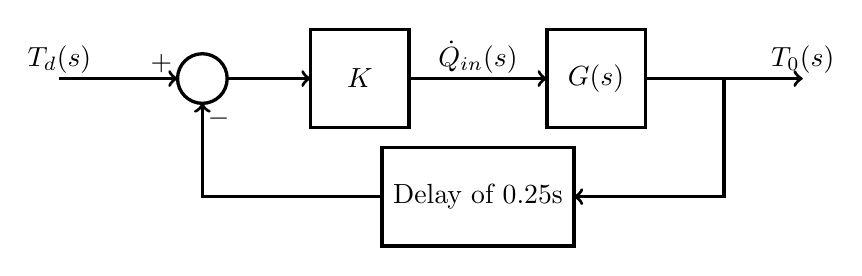
\begin{tikzpicture}[scale=1,inner sep=0pt,outer sep=0pt,very thick,
sysblock/.style={draw,rectangle,inner sep=4pt,minimum width=1.25cm,minimum height=1.25cm,very thick}]

\draw (-2,0) node[draw,circle] (sum1) {$\rule{0pt}{18pt}$};
\draw (0,0) node[sysblock] (C) {$K$};
\draw (3,0) node[sysblock] (G) {$G(s)$};
\draw (1.5,-1.5) node[sysblock] (D) {Delay of 0.25s};

\draw[<-] (sum1.180) node[above left=2pt] {$+$} -- ++(-1.5,0) node[above=2pt] {$T_{d}(s)$};
\draw[->] (sum1.0) --  (C.180);
\draw[->] (C.0) -- node[pos=.5,above=2pt] {$\dot{Q}_{in}(s)$}(G.180);
\draw[->] (G.0) --  ++(2,0) node[above=2pt] {$T_{0}(s)$};
\draw[->] (G.0) -- ++(1,0) |- (D.0);
\draw[->] (D.180) -| (sum1.-90) node[below right=2pt] {$-$};
\end{tikzpicture}
\end{center}



The desired specification is a closed loop step response rise time of 1 second. 

\begin{enumerate}[(a)]
\item Find the transfer function $G(s)$ for the oven from input $\dot{Q}_{in}$ to output $T_{o}$. (We will ignore variations in $T_{a}$ for this problem.) 
\item Using \textsc{Matlab}, plot the Bode plot of $G(s)e^{-s0.25}$, which includes the effect of the delay. (See Section 4 of Lecture 31.)
\item Choose a gain $K$ so that the rise time specification will be met. What is your estimate of the overshoot for the closed loop step response?
\end{enumerate}
